\documentclass{beamer}

\usetheme{Darmstadt}
\usecolortheme{crane}
\usepackage[brazil]{babel}
\usepackage[utf8]{inputenc}
\usepackage[T1]{fontenc}
\usepackage{textcomp}
\usepackage{anyfontsize}
\usepackage[
backend=biber,
style=alphabetic,
citestyle=authoryear
]{biblatex}

\addbibresource{../bib_files/stats.bib}


% Reduced font size
\newcommand\Fontvi{\fontsize{8}{7.2}\selectfont}

% Footnote without number
\newcommand\blfootnote[1]{%
  \begingroup
  \renewcommand\thefootnote{}\footnote{#1}%
  \addtocounter{footnote}{-1}%
  \endgroup
}

\newcommand{\comment}[1]{}

%Information to be included in the title page:
\title[About Beamer] %optional
{Estatística Univariada}

\subtitle{Portal Metabolômica Brasil}

\author[Arthur, Doe] % (optional, for multiple authors)
{R. ~R. ~da Silva\inst{1}}

\institute[VFU] % (optional)
{
  \inst{1}%
  Departamento de Ciências BioMoleculares\\
  Faculdade de Ciências Farmacêuticas

}

\date{\today} % (optional)

\titlegraphic{\includegraphics[width=5.8cm]{../figures/logo_final}} 



\begin{document}

\begin{frame}
\titlepage
\end{frame}

\begin{frame}
\label{contents}
\frametitle{Sumário}
\tableofcontents
\end{frame}

\setbeamercovered{transparent}


\section{Testes de hipóteses}
\setbeamercovered{transparent}
\begin{frame}
\frametitle{Inferência estatística\footcite{magalhaes2002noccoes}}

Na \textbf{inferência estatística} os dois principais objetivos são:

\begin{itemize}
\item
  \textbf{Estimar} um parâmetro populacional

  \begin{itemize}
  \item
    Estimativa pontual
  \item
    Estimativa intervalar
  \end{itemize}
\item
  \textbf{Testar} uma hipótese ou afirmativa sobre um parâmetro
  populacional
\end{itemize}
\blfootnote{\url{http://www.leg.ufpr.br/~paulojus/estbas/}}
\end{frame}

\setbeamercovered{transparent}
\begin{frame}
\frametitle{Testes de hipótese}

\begin{block}{Hipótese}

É uma afirmativa sobre uma propriedade da população

\end{block}

\begin{block}{Teste de hipótese}

\begin{itemize}
\item
  É um procedimento para se testar uma afirmativa sobre uma propriedade
  da população
\item
  Permite tomar \textbf{decisões} sobre a população com base em
  informações de dados amostrais.
\end{itemize}
\end{block}

\end{frame}


\setbeamercovered{transparent}
\begin{frame}
\frametitle{Exemplo 8.1}

Suponha que, entre pessoas sadias, a concentração de certa substância no
sangue se comporta segundo um modelo Normal com média 14 unidades/ml e
desvio padrão 6 unidades/ml.

Pessoas sofrendo de uma doença específica tem concentração média da
substância alterada para 18 unidades/ml.

Admitimos que o modelo Normal com desvio padrão 6 unidades/ml, continua
representado de forma adequada a concentração da substância em pessoas
com a doença.
\end{frame}


\setbeamercovered{transparent}
\begin{frame}
\frametitle{Exemplo 8.1}

\begin{center}\includegraphics[width=0.8\linewidth]{../figures/sadio-doente-1} \end{center}
\end{frame}

\setbeamercovered{transparent}
\begin{frame}
\frametitle{Exemplo 8.1}

Para averiguar se um tratamento é eficaz contra a doença, selecionamos
uma amostra de 30 indivíduos \textbf{submetidos ao tratamento}.

Assumimos que todos os elementos da amostra \(X_1, \ldots, X_{30}\)
possuem a mesma distribuição: \(X_i \sim \text{N}(\mu, 36)\), onde:

\begin{itemize}
\item
  \(\mu = 14\) se o tratamento for eficiente
\item
  \(\mu = 18\) se o tratamento não for eficiente
\end{itemize}

Se a média da amostra for próxima de 14, temos \textbf{evidências} de
que o tratamento é eficaz. Se for mais próxima de 18, as
\textbf{evidências} são contrárias ao tratamento.

Então a pergunta é: o quão próximo é \textbf{``próximo''}?
\end{frame}

\setbeamercovered{transparent}
\begin{frame}
\frametitle{Exemplo 8.1 continuação}

\begin{itemize}
\item
  Interesse geral \(\mu = 14\)?
\item
  Distribuição da média amostral para \(n = 30\):
  \(\text{N}(\mu, 36/30)\).
\item
  Critério para decidir sobre o valor de \(\mu\).
\item
  \textbf{Valor crítico}, digamos \(x_c\) tal que se a média amostral
  (\(\bar{x}_{obs}\)) for maior que \(x_c\) concluímos que a amostra
  pertence a população com média \(18\).
\item
  Como \(\bar{X}\) é uma variável aleatória, devem existir erros
  associados.
\end{itemize}
\end{frame}

\setbeamercovered{transparent}
\begin{frame}
\frametitle{Tipos de hipóteses}

\begin{block}{Hipótese nula \(H_0\)}

É uma afirmativa de que o valor de um parâmetro populacional é
\textbf{igual} a algum valor especificado. (O termo \emph{nula} é usado
para indicar nenhuma mudança, nenhum efeito).

\begin{itemize}
\item
  No ex. 8.1 temos: \(\mu = 14\) unidades/ml
\item
  No ex. 8.2 temos: \(p = 0,4\)
\end{itemize}
\end{block}

\begin{block}{Hipótese alternativa \(H_a\)}

É uma afirmativa de que o parâmetro tem um valor, que, de alguma forma,
difere da hipótese nula. Ex.:

\begin{itemize}
\item
  \(p \neq 0,4\) \qquad \(p < 0,4\) \qquad \(p > 0,4\)
\end{itemize}
\end{block}
\end{frame}


\setbeamercovered{transparent}
\begin{frame}
\frametitle{Tipos de hipóteses}

Quando fazemos um teste de hipótese, chegamos a um dos dois possíveis
resultados:

\begin{itemize}
\item
  \textbf{Rejeitar \(H_0\)}: em favor da hipótese alternativa \(H_a\)
\item
  \textbf{Não rejeitar \(H_0\)}: e conclui-se que não existem diferenças
\end{itemize}

\begin{block}{Atenção!}

\begin{itemize}
\item
  O termo \textbf{aceitar} a hipótese nula é filosoficamente incorreto,
  pois não se pode aceitar uma hipótese baseada apenas em evidências
  amostrais (mesmo em um teste de hipótese formal).
\item
  E ainda existe um \textbf{erro} associado a todo teste de hipótese
\end{itemize}
\end{block}
\end{frame}

\setbeamercovered{transparent}
\begin{frame}
\frametitle{Hipóteses}

\textbf{Hipótese simples}:

\begin{itemize}
\item
  \(H_0:\) O tratamento não é eficaz (\(\mu = 18\))
\item
  \(H_a:\) O tratamento é eficaz (\(\mu = 14\))
\end{itemize}

\textbf{Hipóteses compostas}:

\begin{itemize}
\item
  Hipótese unilateral à esquerda

  \begin{itemize}
  \item
    \(H_0:\) O tratamento não é eficaz (\(\mu = 18\));
  \item
    \(H_1:\) O tratamento é eficaz (\(\mu < 18\)).
  \end{itemize}
\item
  Hipótese bilateral:

  \begin{itemize}
  \item
    \(H_0:\) O tratamento não é eficaz (\(\mu = 18\));
  \item
    \(H_1:\) O tratamento é eficaz (\(\mu \neq 18\)).
  \end{itemize}
\end{itemize}
\end{frame}

\setbeamercovered{transparent}
\begin{frame}
\frametitle{Erros ao realizar um teste de hipótese}

\begin{center}\includegraphics[width=0.7\linewidth]{../img/errors} \end{center}
\end{frame}

\setbeamercovered{transparent}
\begin{frame}
\frametitle{Erros ao realizar um teste de hipótese}

\begin{itemize}
\item
  \textbf{Erro Tipo I}: rejeitar \(H_0\), quando \(H_0\) é verdadeira.
\item
  \textbf{Erro Tipo II}: não rejeitar \(H_0\) quando \(H_0\) é falsa.
\end{itemize}

\begin{table}[h]
\centering
\begin{tabular}{c|cc}
\hline
& \textbf{$H_o$ verdadeira} & \textbf{$H_o$ falsa} \\
\hline
\textbf{Não rejeitar $H_0$} & Decisão correta & Erro tipo II \\
\textbf{Rejeitar $H_0$} & Erro tipo I & Decisão correta \\
\hline
\end{tabular}
\end{table}
\end{frame}

\setbeamercovered{transparent}
\begin{frame}
\frametitle{Erros ao realizar um teste de hipótese}

Definimos por \(\alpha\) e \(\beta\) as probabilidades de cometer os
erros do tipo I e II:

\begin{itemize}
\item
  \(\alpha = P(\text{erro tipo I}) = P(\text{rejeitar } H_0 \, | \, H_0 \text{ verdadeira})\)
\item
  \(\beta = P(\text{error tipo II}) = P(\text{não rejeitar } H_0 \, | \, H_0 \text{ falsa})\)
\end{itemize}

No exemplo 8.1, se \(H_0: \mu = 18\) e \(H_a: \mu < 18\), então:

\begin{itemize}
\item
  \(\alpha = P(\text{concluir que o tratamento é eficaz quando na verdade não é})\)
\item
  \(\beta = P(\text{concluir que o tratamento não é eficaz quando na verdade é})\)
\end{itemize}
\end{frame}

\setbeamercovered{transparent}
\begin{frame}
\frametitle{Erros ao realizar um teste de hipótese}

\begin{center}\includegraphics[width=0.8\linewidth]{../figures/erro1-1} \end{center}
\end{frame}

\setbeamercovered{transparent}
\begin{frame}
\frametitle{Erros ao realizar um teste de hipótese}

\begin{center}\includegraphics[width=0.8\linewidth]{../figures/erro2-1} \end{center}
\end{frame}

\setbeamercovered{transparent}
\begin{frame}
\frametitle{Erros ao realizar um teste de hipótese}

A situação ideal é aquela em que ambas as probabilidades, \(\alpha\) e
\(\beta\), são próximas de zero.

No entanto, à medida que diminuimos \(\alpha\), a probabilidade
\(\beta\) tende a aumentar.

Levando isso em conta, ao formular as hipóteses, \textbf{devemos cuidar
para que o erro mais importante a ser evitado seja o erro do tipo I}.

Por isso, a probabilidade \(\alpha\) recebe o nome de \textbf{nível de
significância} do teste, e é esse erro que devemos controlar.
\end{frame}

\setbeamercovered{transparent}
\begin{frame}
\frametitle{Valor crítico}

Supondo \(\alpha\) conhecido podemos determinar o valor crítico \(x_c\).
\begin{align*}
\alpha &= P(\text{erro tipo I}) = P(\text{rejeitar } H_0 \, | \, H_0
\text{ verdadeira}) \\
 &= P(\bar{X} < x_c \, | \, \mu = 18) = P\left( \frac{\bar{X} -
 \mu}{\sigma/\sqrt{n}} < \frac{x_c - 18}{6/\sqrt{30}} \right) \\
 &= P(Z < z_c)
\end{align*}

com \(Z \sim N(0,1)\).
\end{frame}

\setbeamercovered{transparent}
\begin{frame}
\frametitle{Obtendo o valor crítico}

Dado \(\alpha\) encontramos \(z_c\) na tabela normal padrão.

Obtemos \(x_c\) \[
z_c = \frac{x_c - 18}{6/\sqrt{30}} \quad \Rightarrow \quad x_c = 18 +
z_c \frac{6}{\sqrt{30}}
\]

Supondo \(\alpha = 0.05\) temos \[
0.05 = P(Z < z_c) \quad \Rightarrow \quad z_c = -1.64
\] logo \[
x_c = 18 - 1.64 \frac{6}{\sqrt{30}} = 16.2
\]
\end{frame}

\setbeamercovered{transparent}
\begin{frame}
\frametitle{Região Crítica}

Dada uma amostra, se \(\bar{x}_{obs} < 16.2\), \textbf{rejeitamos}
\(H_0\), concluindo que o tratamento é eficaz.

O conjunto dos números reais menores que 16.2 é denominado de
\textbf{Região de Rejeição} ou \textbf{Região Crítica} (RC), isto é: \[
RC = \{ x \in \mathbb{R} : x < 16.2 \}.
\] \textbf{No exemplo 8.1}, se a média amostral dos 30 indivíduos foi
\(\bar{x}_{obs} = 16.04\), então \textbf{rejeitamos} \(H_0\), ao nível
de significância \(\alpha = 0.05\).

Nesse caso, \(\bar{x}_{obs} < x_c\) está dentro da RC.
\end{frame}


\setbeamercovered{transparent}
\begin{frame}
\frametitle{Região Crítica}

\begin{center}\includegraphics[width=0.8\linewidth]{../figures/rc-1} \end{center}
\end{frame}

\setbeamercovered{transparent}
\begin{frame}
\frametitle{Teste de hipótese bilateral}

Definindo as hipóteses \[
H_0: \mu = \mu_0 \quad \text{e} \quad H_a: \mu \neq \mu_0
\] A Região Crítica será dada por \[
RC = \{x \in \mathbb{R} \, | \, x < x_{c_1} \quad \text{ou} \quad x >
x_{c_2} \}
\] Para um valor de \(\alpha\) fixado, determinamos \(x_{c_1}\) e
\(x_{c_2}\) de modo que \[
P(\bar{X} < x_{c_1} \cup \bar{X} > x_{c_2}) = \alpha
\] Assim, distribuimos a área \(\alpha\) igualmente entre as duas partes
da RC \[
P(\bar{X} < x_{c_1}) = \frac{\alpha}{2} \quad \text{e} \quad P(
\bar{X} > x_{c_2}) = \frac{\alpha}{2}
\]
\end{frame}

\setbeamercovered{transparent}
\begin{frame}
\frametitle{Teste de hipótese bilateral}


\begin{center}\includegraphics[width=0.8\linewidth]{../figures/rc2-1} \end{center}
\end{frame}

\setbeamercovered{transparent}
\begin{frame}
\frametitle{Etapas de um teste de hipótese}

\begin{enumerate}
\def\labelenumi{\arabic{enumi}.}
\item
  Estabelecer as hipóteses nula e alternativa.
\item
  Definir a forma da região crítica, com base na hipótese alternativa.
\item
  Identificar a distribuição do estimador e obter sua estimativa.
\item
  Fixar \(\alpha\) e obter a região crítica.
\item
  Concluir o teste com base na estimativa e na região crítica.
\end{enumerate}
\end{frame}

\setbeamercovered{transparent}
\begin{frame}
\frametitle{\(P\)-valor}

Em geral, \(\alpha\) é pré-fixado para construir a regra de decisão.

Uma alternativa é deixar em aberto a escolha de \(\alpha\) para quem for
tomar a decisão.

A ideia é calcular, \textbf{supondo que a hipótese nula é verdadeira}, a
probabilidade de se obter estimativas mais extremas do que aquela
fornecida pela amostra.

Essa probabilidade é chamada de \textbf{nível descritivo}, denotada por
\(\alpha^*\) (ou \(P\)-valor).

Valores pequenos de \(\alpha^*\) evidenciam que a hipótese nula é falsa.

O conceito de ``pequeno'' fica para quem decide qual \(\alpha\) deve
usar para comparar com \(\alpha^*\).
\end{frame}

\setbeamercovered{transparent}
\begin{frame}
\frametitle{\(P\)-valor}

Para \textbf{testes unilaterais}, sendo \(H_0: \mu = \mu_0\), a
expressão de \(\alpha^*\) depende da hipótese alternativa:
\begin{align*}
\alpha^* &= P(\bar{X} < \bar{x}_{obs} \, | \, H_0 \text{ verdadeira}) \quad
\text{para } H_a: \mu < \mu_0 \\
\alpha^* &= P(\bar{X} > \bar{x}_{obs} \, | \, H_0 \text{ verdadeira}) \quad
\text{para } H_a: \mu > \mu_0
\end{align*} Para \textbf{testes bilaterais}, temos \(H_0: \mu = \mu_0\)
contra \(H_0: \mu \neq \mu_0\), a definição do nível descritivo depende
da relação entre \(\bar{x}_{obs}\) e \(\mu_0\): \begin{align*}
\alpha^* &= 2 \times P(\bar{X} < \bar{x}_{obs} \, | \, H_0 \text{
verdadeira}) \quad \text{se }  \bar{x}_{obs} < \mu_0 \\
\alpha^* &= 2 \times P(\bar{X} > \bar{x}_{obs} \, | \, H_0 \text{
verdadeira}) \quad \text{se }  \bar{x}_{obs} > \mu_0 \\
\end{align*} Como estamos calculando a probabilidade para apenas uma das
caudas, então esse valor é multiplicado por 2.
\end{frame}


\section{Comparação entre 2 populações}
\setbeamercovered{transparent}
\begin{frame}
\frametitle{Comparação de Duas Médias}

Duas das principais suposições feitas no desenvolvimento dos testes de hipóteses foram:

\begin{itemize}
\item
  Independência entre os componentes da amostra;
\item
  Variabilidade associada aos valores populacionais e amostrais.
\end{itemize}

\begin{block}{Testes Paramétricos}
Os testes paramétricos discutidos aqui, assumem variáveis que se comportam segundo modelo Normal, ou que as amostras são suficientemente grandes para obter uma aproximação.
\end{block}
\end{frame}


\setbeamercovered{transparent}
\begin{frame}
\frametitle{Comparação de Duas Médias}

\begin{center}\includegraphics[width=1.1\linewidth]{../img/figure_9_1} \end{center}
\end{frame}

\subsection{Amostras independentes}
\setbeamercovered{transparent}
\begin{frame}
\frametitle{Amostras independentes com variâncias conhecidas}

Consideramos agora o teste relacionado com a situação em que queremos comparar médias de duas populações independentes, quando as correspondentes variâncias são conhecidas. A obtenção de informação a respeito do valor de variância populacional pode ser obtido de estudos anteriores ou experimentos similares. \\~\\

Supondo duas populações com variâncias iguais a um valor conhecido \(\sigma^2_0\). Além disso, adimitamos que as populações seguem uma distribuição Normal, com médias \(\mu_1\) e \(\mu_2\). Obtendo amostras aleatórias independentes \((X_1, ..., X_{n1})\) e \((Y_1, ..., Y_{n2})\) de cada população com, tamanhos \(n_1\) e \(n_2\) para as duas amostras, podemos testar as seguintes hipóteses:

\begin{align*}
H_0 &: \mu_1 = \mu_2  \\
H_a &: \mu_1 \neq \mu_2
\end{align*}   


\end{frame}


\setbeamercovered{transparent}
\begin{frame}
\frametitle{Amostras independentes com variâncias conhecidas}

Como estamos interessados em determinar se a diferença é estatisticamente significante, podemos ainda reescrever as hipóteses em termos de \(\mu_D = \mu_1-\mu_2\), isto é: \begin{align*}
H_0 &: \mu_D = 0 & \text{(As médias populacionais são iguais;)} \\
H_a &: \mu_D \neq 0 & \text{(As médias populacionais não são iguais;),}
\end{align*}
o que sugere trabalharmos com o \textit{estimador} de \(\mu_D\):
\begin{align*}
\bar{D} = \bar{X}-\bar{Y}
\end{align*}
Com as suposições feitas, temos
\begin{align*}
X_i \sim N(\mu_1, \sigma^2_0), i = 1,2, \ldots, n_1; \\
Y_i \sim N(\mu_2, \sigma^2_0), i = 1,2, \ldots, n_2;
\end{align*}

\end{frame}


\setbeamercovered{transparent}
\begin{frame}
\frametitle{Amostras independentes com variâncias conhecidas}

Pela independência dessa variáveis, \(\bar{D}\) terá distribuição Normal com média \(E(\bar{D})=\mu_D\) e quanto à variância, temos:
\begin{align*}
Var(\bar{D}) &= Var(\bar{X}-\bar{Y}) = Var(\bar{X}) + Var(\bar{Y}) \\
             &= \frac{\sigma^2_0}{n_1}+\frac{\sigma^2_0}{n_2} = \sigma^2_0(\frac{1}{n_1}+\frac{1}{n_2})
\end{align*}

Note que a independência entre as amostras foi necessária para obter essa variância.

\end{frame}

\setbeamercovered{transparent}
\begin{frame}
\frametitle{Resumo}

\textbf{Tabela 9.1: Comparação de médias para duas populações}

\begin{table}[h]
\tiny
\begin{tabular}{|c|c|}
\hline
Situação  & Estimadores  \\
\hline
Amostras Pareadas (Caso 1)  & 
\parbox{1cm}{\begin{align*}
\bar{D} &= \frac{\sum_i^nD_i}{n} \\
S^2_D &= \frac{1}{n-1}\sum_{i=1}^n(D_i-\bar{D})^2 \\
T &= \frac{\bar{D}-\mu_D}{S_D/\sqrt{n}} \sim t_{(n-1)}
\end{align*}}  \\
\hline
Amostras Independentes (Caso 2) Variâncias conhecidas  & 
\parbox{1cm}{\begin{align*}
\bar{D} &= \bar{X}-\bar{Y} \\
Var(\bar{D}) &= \sigma^2_X/n_1 + \sigma^2_Y/n_2 \\
Z &= \frac{\bar{D}-\mu_D}{\sqrt{\sigma^2_X/n_1 + \sigma^2_Y/n_2}}
\end{align*}} \\
\hline
\end{tabular}
\end{table}
\end{frame}

\setbeamercovered{transparent}
\begin{frame}
\frametitle{Resumo}
\textbf{Tabela 9.1: Comparação de médias para duas populações}
\begin{table}[h]
\tiny
\begin{tabular}{|c|c|}
\hline
Situação  & Estimadores  \\
\hline
Amostras Independentes (Caso 3A) Variâncias desconhecidas e iguais  &  \parbox{1cm}{\begin{align*}
\bar{D} &= \bar{X}-\bar{Y} \\
S^2_c &= \frac{(n_1-1)S^2_X+(n_2-1)S^2_Y}{(n_1-1)+(n_2-1)} \\
T &= \frac{\bar{D}-\mu_D}{\sqrt{S^2_c(1/n_1 + 1/n_2)}}
\end{align*}} \\
\hline
Amostras Independentes (Caso 3B) Variâncias desconhecidas e diferentes  & \parbox{1cm}{\begin{align*}
\bar{D} &= \bar{X}-\bar{Y} \\
\hat{\sigma}_{\bar{D}}^2 &= S^2_X/n_1+S^2_Y/n_2 \\
T &= \frac{\bar{D}-\mu_D}{\sqrt{S^2_X/n_1+S^2_Y/n_2}}
\end{align*}}  \\
\hline

\end{tabular}
\end{table}
\end{frame}

\section{Análise de Variância}
\setbeamercovered{transparent}
\begin{frame}
\frametitle{Análise de Variância}
Consideramos nesta seção o caso de comparação de três ou mais populações, definidas por uma variável qualitativa (fator) através de testes com as correspondentes médias. Iniciamos com o caso em que as amostras de cada população têm o mesmo tamanho. \\~\\

Consideraremos um modelo estatístico, em que cada observação \(Y\) pode ser decomposta em duas componentes: \textit{sistemática} e \textit{aleatória}, esta última representando variações individuais e todos os fatores que não são explicados pela parte sistemática. Matematicamente, podemos escrever

\begin{align*}
Y = \mu+e.
\end{align*}
 
\end{frame}


\setbeamercovered{transparent}
\begin{frame}
\frametitle{Análise de Variância}
Se \(Y\) representa a observação associada a uma unidade experimental, a parte sistemática \(\mu\) pode ser vista como média populacional, que é fixa, e a parte aleatória \textit{\textbf{e}} como a informação referente a outros fatores que podem influir nas observações mas não são incorporadas em \(\mu\). \\~\\


Suponha que estamos interessados em compara as médias de \(K\) populações, isto é, queremos testar

\begin{align*}
H_0 &: \mu_1 = \mu_2 = \ldots = \mu_K;  \\
H_a &: \text{pelo menos uma das médias \(\mu_i\) é diferente das demais.}
\end{align*}
 
\end{frame}

\setbeamercovered{transparent}
\begin{frame}
\frametitle{Análise de Variância}
Definimos as quantidades \textit{Soma de Quadrados Dentro} (SQD)

\begin{align*}
SQD = \sum_{i=1}^K\sum_{j=1}^m(Y_{ij}-\hat{\mu}_i)^2 = \sum_{i=1}^K\sum_{j=1}^m(Y_{ij}-\bar{Y}_i)^2 = \sum_{i=1}^K\sum_{j=1}^mY_{ij}^2-m\sum_{i=1}^K\bar{Y}_i^2;  
\end{align*}

e \textit{Soma de Quadrados Total} (SQT)

\begin{align*}
SQT = \sum_{i=1}^K\sum_{j=1}^m(Y_{ij}-\hat{\mu})^2 = \sum_{i=1}^K\sum_{j=1}^m(Y_{ij}-\bar{Y})^2 = \sum_{i=1}^K\sum_{j=1}^mY_{ij}^2-mK\bar{Y}^2.  
\end{align*}

\end{frame}


\setbeamercovered{transparent}
\begin{frame}
\frametitle{Análise de Variância}
A diferença entre SQT e SQD representa a \textit{soma de quadrados entre} será denotada por SQE, isto é,

\begin{align*}
SQE = SQT-SQD.
\end{align*}

Das expressões para soma de quadrados total e de dentro, segue que:

\begin{align*}
SQE = m\sum_{i=1}^K(\bar{Y}_{i}-\bar{Y})^2 = m(\sum_{i=1}^K\bar{Y}^2_{i}-K\bar{Y}^2).  
\end{align*}

\end{frame}

\setbeamercovered{transparent}
\begin{frame}
\frametitle{Análise de Variância}
Cada uma das somas de quadrados envolve um certo número de quantidades que estão sendo estimadas. Por exemplo, SQT contém \(\bar{Y}\) e SQD contém \(\bar{Y}_i\), \(i=1,\ldots,K\). Levando este fato em consideração e o número de observações nas amostras, definimos os correspondentes quadrados médios:

\begin{align*}
QMT = \frac{SQT}{Km-1} &: \text{quadrado médio total}; \\
QMD = \frac{SQD}{Km-K} = \frac{SQD}{K(m-1)} &: \text{quadrado médio dentro}; \\
QME = \frac{SQE}{K-1} &: \text{quadrado médio entre.}
\end{align*}

Note que, nesse caso, é preciso calcular as três quantidades anteriores pois QMT não é igual à soma de QMD com QME.

\end{frame}


\setbeamercovered{transparent}
\begin{frame}
\frametitle{Análise de Variância}
O teste estatístico para hipótese \(H_0\) envolve os quadrados médios. Se QME for grande comparado à QMD, a parte sistemática do modelo estará captando grande parte da informação dos dados e a hipótese \(H_0\) deverá ser rejeitada. Definimos, então, a quantidade

\begin{align*}
F = \frac{QME}{QMD}.
\end{align*}

\end{frame}

\setbeamercovered{transparent}
\begin{frame}
\frametitle{Análise de Variância}
Temos, agora condições de encontrar o valor crítico de \(f_c\) e determinar a região crítico do teste, que será da forma

\begin{align*}
RC = \{f \in \mathbb{R}^+ \, : \, f > f_c \}
\end{align*}

Das três suposições feitas, a mais importante é a segunda, \(Var(Y_{ij}) = \sigma^2\), para \(i=1,\ldots,K\) e \(j=1,\ldots,m\), que tem o nome técnico de \textit{homocedasticidade}. 
 
\end{frame}


\setbeamercovered{transparent}
\begin{frame}
\frametitle{Análise de Variância}
A discussão sobre o comportamento dos erros e das somas de quadrados é resumida na \textbf{Tabela de Análise de Variância (ANOVA)} Tabela 9.2:

\begin{table}[h]
\centering
\begin{tabular}{ccccc}
\hline
Fonte de & Graus de & Soma de & Quadrado & F  \\
Variação & Liberdade & Quadrados & Médio &   \\
\hline
Entre & K-1 & SQE & QME & QME/QMD   \\
Dentro & K(m-1) & SQD & QMD &   \\
\hline
Total & Km-1 & SQT &  &   \\
\hline
\end{tabular}

\end{table}
\end{frame}

\section{Comparações múltiplas de hipótese}
\setbeamercovered{transparent}
\begin{frame}
\frametitle{Métodos de comparações múltiplas de hipótese}

\begin{itemize}
\item São aplicadas após a rejeição de \(H_0\) pela estatística F da ANOVA;
\item São métodos para corrigir a inflação do nível de significância global decorrene do teste de um grande número de hipótese; 
\item Isso é feito principalmente de duas formas:
\begin{enumerate}
\item Corrige-se o p-valor após os testes de hipótese individuais para ter nível de significância global \(\alpha_k\) desejado.
\item Emprega-se uma estatística de teste de hipótese que incorpore o número de hipóteses para ter nível de significância global \(\alpha_k\) desejado.
\end{enumerate}
\end{itemize}

\end{frame}

\setbeamercovered{transparent}
\begin{frame}
\frametitle{Correção do p-valor pelo método de Bonferroni}

\begin{itemize}
\item Agora serão testadas separadamente um conjunto de hipóteses
\[H_0: m_i = m_j \quad \forall \quad i \neq j\]
\item Se as hipóteses forem para todos os pares possíveis de \(i, j \in \{1; \ldots; k\}\), já foi visto que totalizam \(u = \binom{k}{2}\).
\item Dado um nível de significância global, para \textit{p} hipóteses independentes, o nível de significância individual \(\alpha\) corrigido é
\[\alpha_p=1-(1-\alpha)^p\quad logo\]
\[\alpha = 1-(1-\alpha_p)^{1/p} \approx \alpha_p/p\]
\item Dessa forma, o p-valor do teste t individual é multiplicado por p para corrigir pela quantidade de hipóteses. 
\end{itemize}

\end{frame}

\setbeamercovered{transparent}
\begin{frame}
\frametitle{Método de Benjamini–Hochberg}

\begin{itemize}
\item Testando \textit{m} hipóteses
\[H_1, H_2, \ldots, H_m\]
\item Os \textit{Valores-P}
\[p_1, p_2, \ldots, p_m\]
\item Ordenar os \textit{Valores-P}
\[p_{(1)} \leq p_{(2)} \leq \ldots \leq p_{(m)}\]
\item Seja \(\alpha\) a taxa de falsas descobertas (FDR) que se quer controlar, encontre
\[p_{(i)} \leq \frac{i}{m}\alpha\]
\item Faça o Valor-P correspondente o ponto de corte, a taxa FDR está controlada em \(\alpha\). 
\end{itemize}
\blfootnote{\url{https://en.wikipedia.org/wiki/False_discovery_rate}}
\end{frame}

\setbeamercovered{transparent}
\begin{frame}
\frametitle{Comparações múltiplas pelo teste de Tukey}

\begin{itemize}
\item Outra opção é trocar a estatística de teste \(\Rightarrow\) outra distribuição amostral.
\item Pelo teste de Tukey, rejeita-se a hipótese de igualdade de duas médias quando
\[q_0 = \frac{abs(\bar{y}_i-\bar{y}_j)}{ep(\bar{y}_i-\bar{y}_j)}=\frac{abs(\bar{y}_i-\bar{y}_j)}{\sqrt{2s^2/r}} > q_{\alpha, \nu, k},\]
em que \(q_{\alpha, \nu, k}\) é o quantil superior da distribuição da amplitude total studentizada e ep(.) denota o erro padrão.
\item Ou seja, não se usa mais a distribuição t mas sim esta que incorpora o número de tratamentos (k) como parâmetro.
\item Pelo uso desta estatística de teste se faz o controle para manter o nível de significância global no valor desejado. 
\end{itemize}

\end{frame}

\setbeamercovered{transparent}
\begin{frame}
\frametitle{Pressuposições}
As pressuposições gerais de testes paramétricos são:
\begin{itemize}
\item As populações sendo comparadas são normalmente distribuidas.
\item A amostra é representativa da população.
\item Os dados estão em uma escala intervalar ou proporcional.
\end{itemize}
Teste não paramétricos podem ser usados quando:
\begin{itemize}
\item Os dados não se ajustam a uma distribuição especificada e pressuposições não são feitas.
\item Dados são medidos em qualquer escala.
\end{itemize}


\end{frame}

\setbeamercovered{transparent}
\begin{frame}
\frametitle{Pressuposições}

\begin{itemize}
\item Pode-se inspecionar os pressupostos pela análise de resíduos.
\item Também é possível aplicar testes de hipótese para os pressupostos.
\item Os pressupostos não devem ser violados para a validade das inferências.
\end{itemize}

\end{frame}

\setbeamercovered{transparent}
\begin{frame}
\frametitle{Qual teste aplicar?\footcite{vinaixa2012guideline}}

\begin{table}[h]
\fontsize{9pt}{9pt}\selectfont
\centering
\begin{tabular}{ccc}
\hline
 Desenho Experimental & Distribuição Normal & Distribuição Não Normal    \\
\hline
 &  Compare médias & Compare medianas   \\
Dados não pareados & Teste-t & Mann-Whitney   \\
Dados pareados & Teste-t pareado & Wilcoxon \\
>2 grupos não pareados & Anova & Kruskal-Wallis \\
>2 grupos pareados & Anova - medidas repetidas & Friedman \\
\hline
\end{tabular}

\end{table}
\end{frame}

\setbeamercovered{transparent}
\begin{frame}
\frametitle{Fluxo de análises completo}

\begin{center}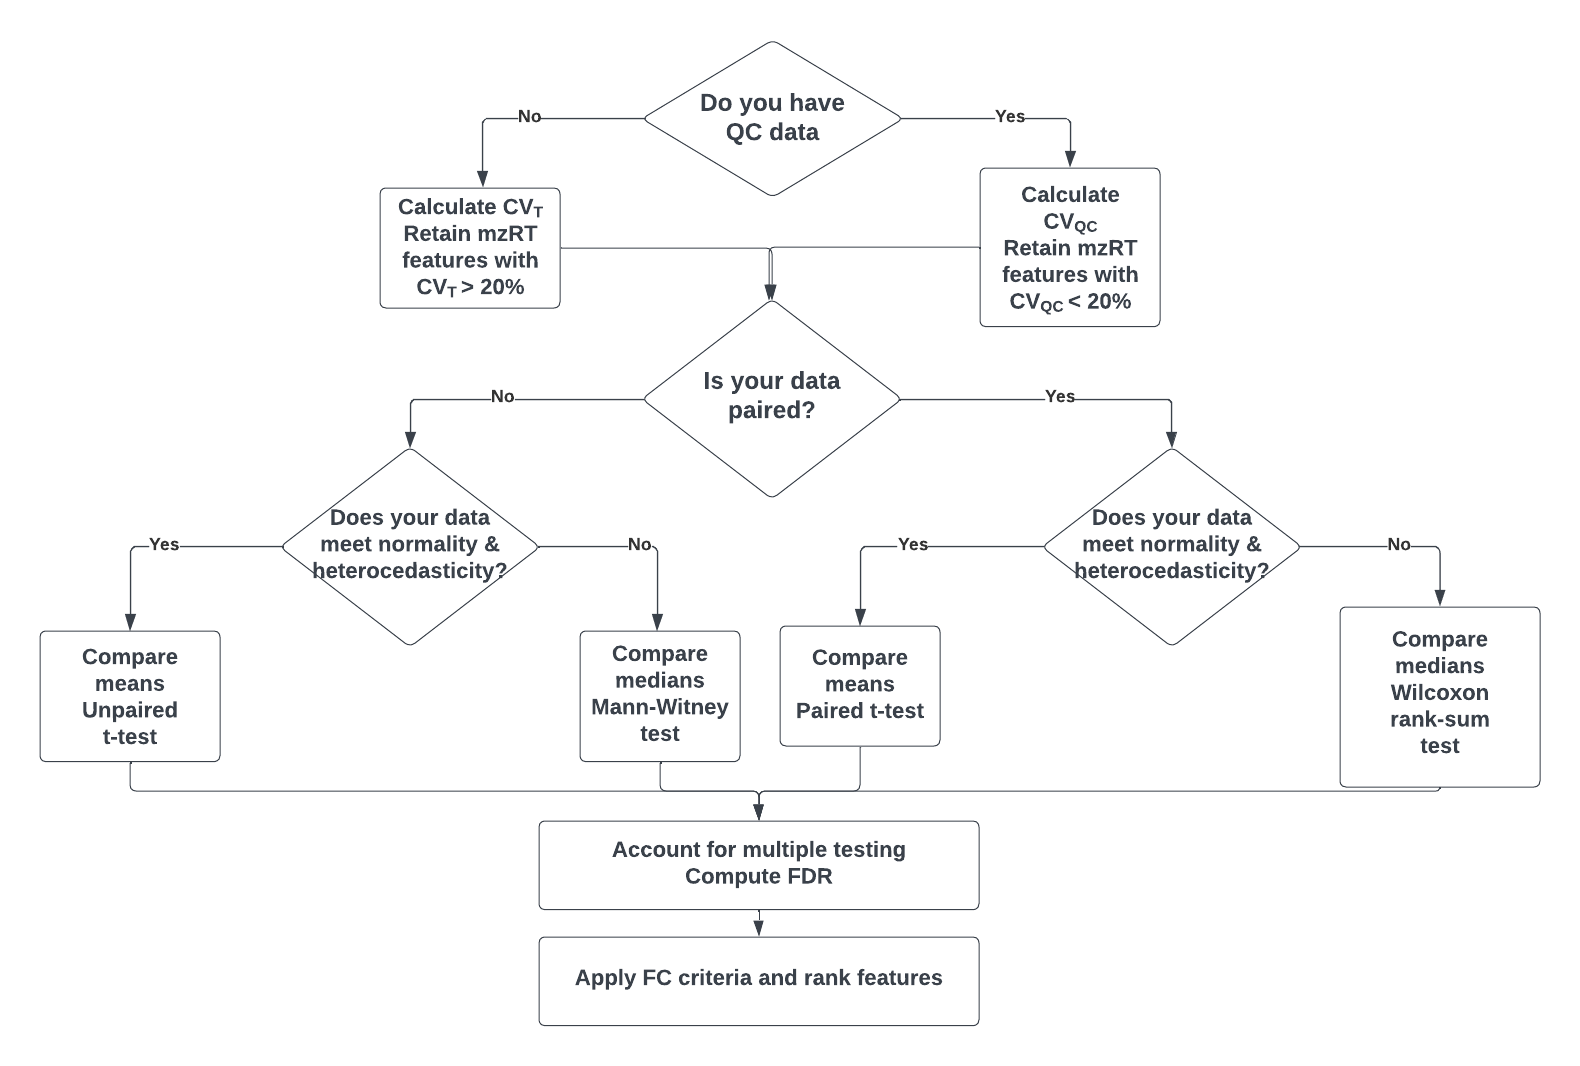
\includegraphics[width=1\linewidth]{../figures/workflow} \end{center}
\end{frame}

\section{Volcano plot}
\setbeamercovered{transparent}
\begin{frame}
\frametitle{Volcano plot}
Um gráfico de \textit{Volcano} é um tipo de gráfico de dispersão usado para identificar rapidamente mudanças em grandes conjuntos de dados. Suas principais características são

\begin{itemize}
\item Representa graficamente a significância versus a magnitude da diferença em y e x, respectivamente.
\item Usa o negativo do logaritmo do valor p no eixo y (geralmente na base 10).
\item O logaritmo da razão entre as médias dos grupos comparados (geralmente na base 2) é utilizano no eixo x. 
\end{itemize}

\blfootnote{\url{https://en.wikipedia.org/wiki/Volcano_plot_(statistics)}}
\end{frame}

\setbeamercovered{transparent}
\begin{frame}
\frametitle{Volcano plot}

\begin{center}\includegraphics[width=0.8\linewidth]{../figures/Volcano_eg} \end{center}
\end{frame}

\setbeamercovered{transparent}
\begin{frame}
\frametitle{Referências bibliográficas}
\printbibliography
\end{frame}

\end{document}